\begin{center}
    \vspace*{1.5cm}
    {\fontsize{20}{20}\textbf{Slaskvisor}}\\
    \vspace{0.7cm}
    {\fontsize{12}{12}\textit{Om drägget själv får välja}}
\end{center}
\addtocwithheader{Slaskvisor}  % Add entry to TOC and set header\noBackground
\noBackground

\newpage
\noBackground

% ----- GAMLA BAMSE -----
%\begin{textblock*}{3cm}(6.0cm,2.5cm) % {width}(x, y)
%    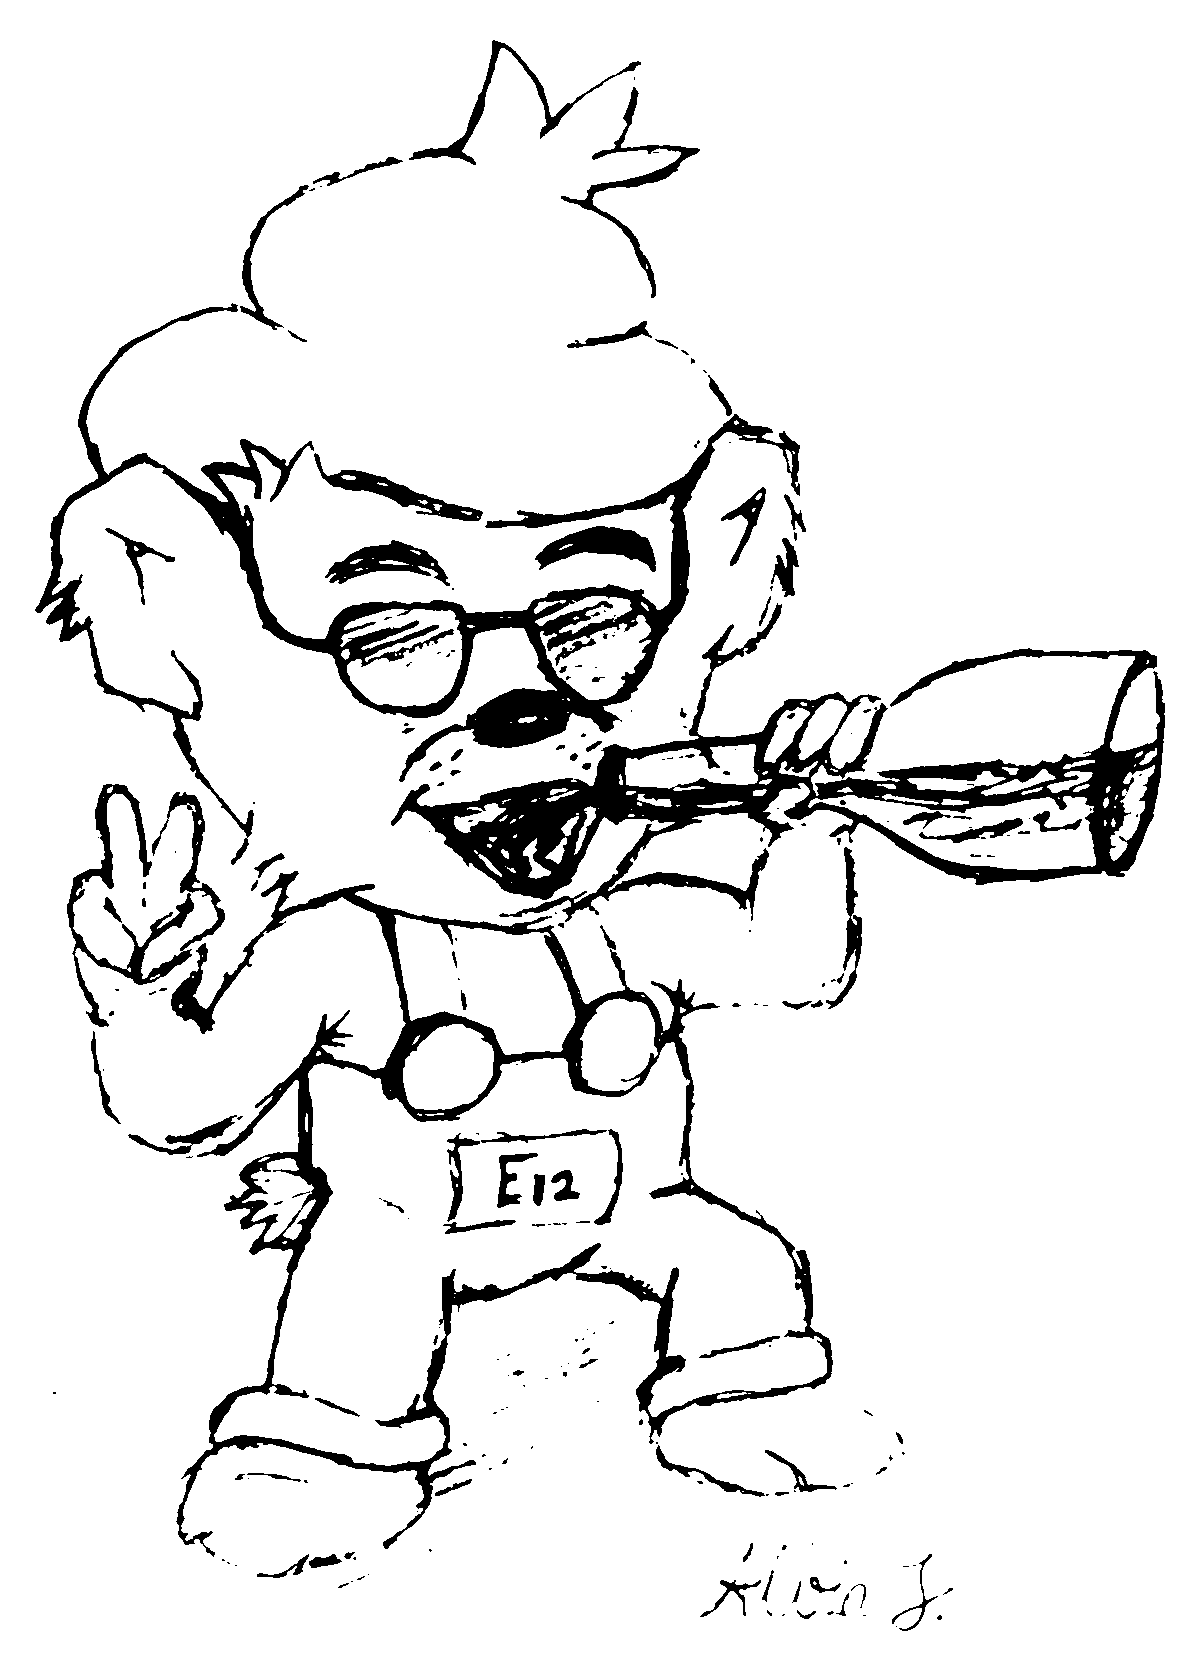
\includegraphics[width=4.7cm]{./bilder/bamse.png}
%\end{textblock*}

% ----- NYA BAMSE -----
\begin{comment}
\begin{textblock*}{3cm}(5.5cm,3.2cm) % {width}(x, y)
    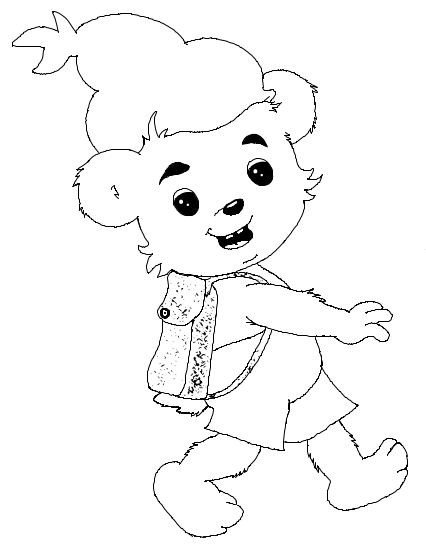
\includegraphics[width=2.8cm]{./bilder/majas-bilder/bamse-1.png}
\end{textblock*}

\begin{textblock*}{3cm}(7.6cm,6.7cm) % {width}(x, y)
    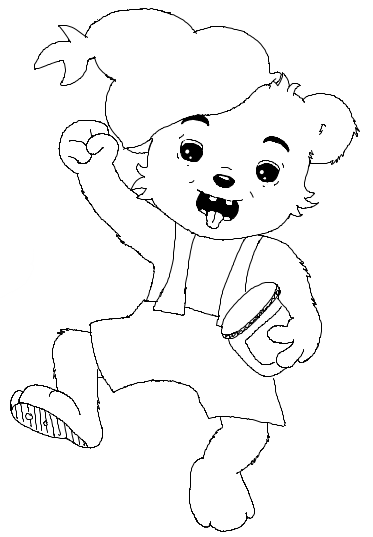
\includegraphics[width=2.6cm]{./bilder/majas-bilder/bamse-2.png}
\end{textblock*}

\begin{textblock*}{3cm}(5.6cm,10.2cm) % {width}(x, y)
    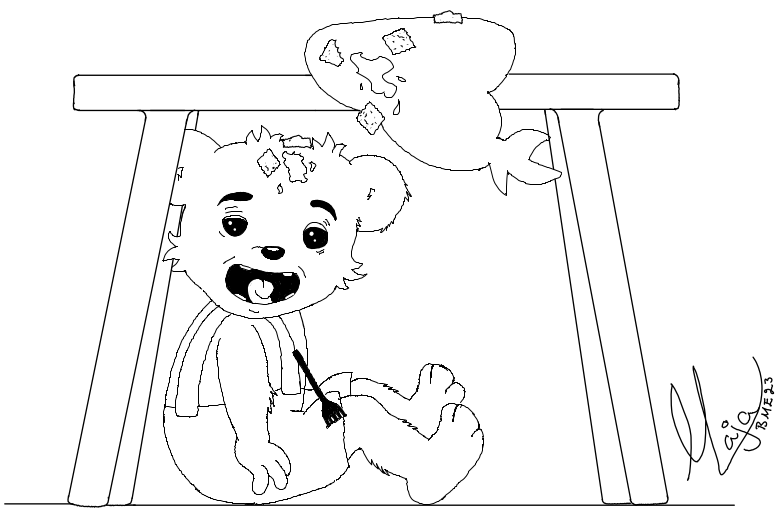
\includegraphics[width=4.9cm]{./bilder/majas-bilder/bamse-3.png}
\end{textblock*}


\begin{textblock*}{3cm}(7cm,2cm) % {width}(x, y)
    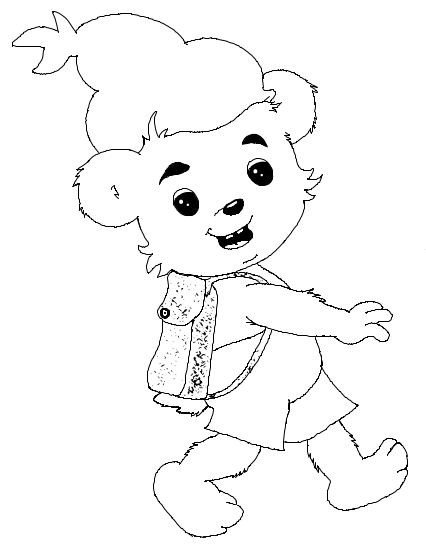
\includegraphics[width=3.2cm]{./bilder/majas-bilder/bamse-1.png}
\end{textblock*}

\begin{textblock*}{3cm}(6 cm,5.5cm) % {width}(x, y)
    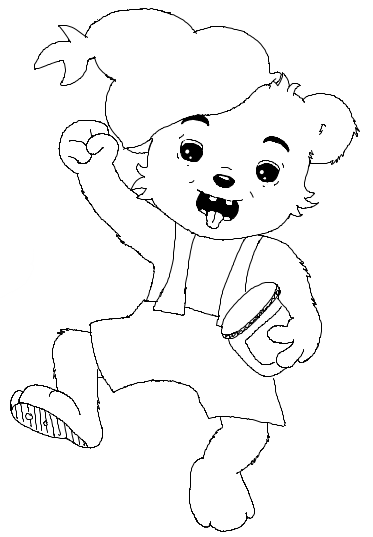
\includegraphics[width=2.8cm]{./bilder/majas-bilder/bamse-2.png}
\end{textblock*}

\begin{textblock*}{3cm}(6cm,9.4cm) % {width}(x, y)
    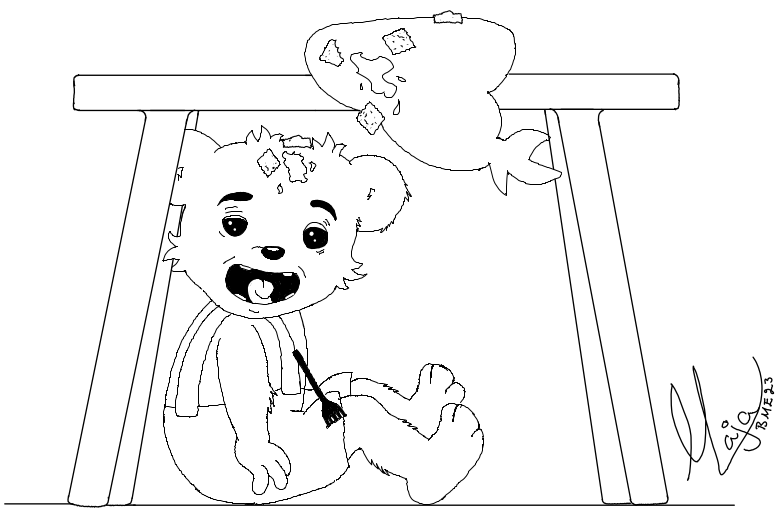
\includegraphics[width=4.9cm]{./bilder/majas-bilder/bamse-3.png}
\end{textblock*}


\begin{textblock*}{3cm}(7.6 cm, 3.2cm) % {width}(x, y)
    %\scalebox{-1}[1]{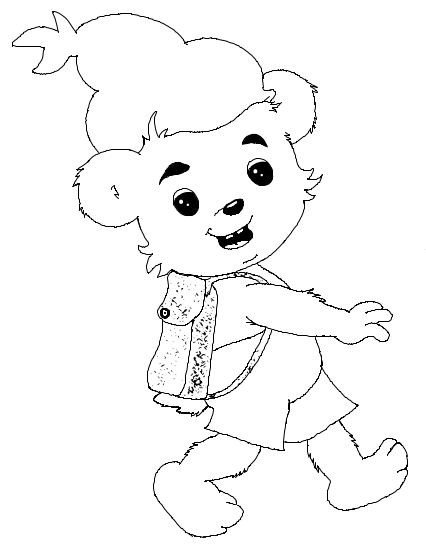
\includegraphics[width=2.4cm]{./bilder/majas-bilder/bamse-1.png}}
    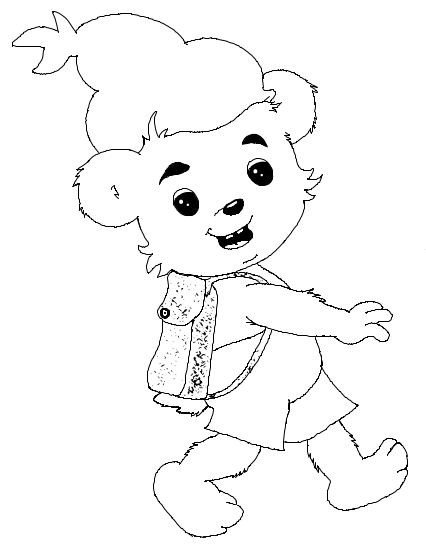
\includegraphics[width=2.4cm]{./bilder/majas-bilder/bamse-1.png}
\end{textblock*}

\begin{textblock*}{3cm}(6.6cm, 6cm) % {width}(x, y)
    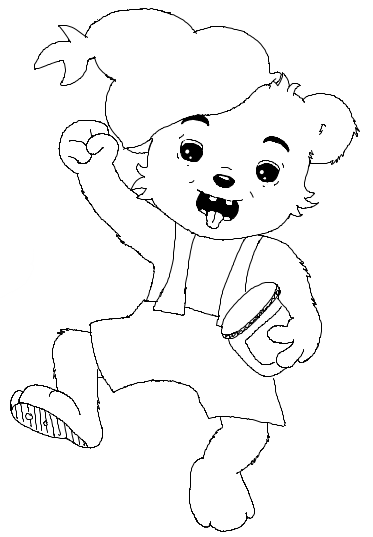
\includegraphics[width=2.2cm]{./bilder/majas-bilder/bamse-2.png}
\end{textblock*}

\begin{textblock*}{3cm}(6.6cm,9.3cm) % {width}(x, y)
    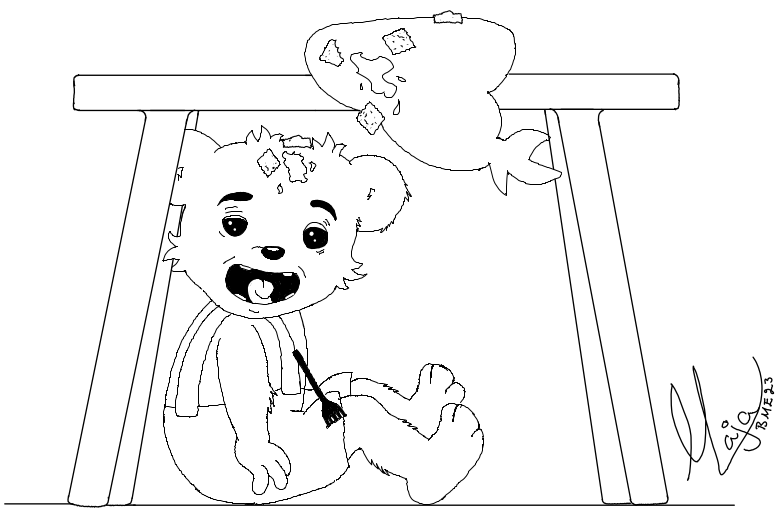
\includegraphics[width=3.8cm]{./bilder/majas-bilder/bamse-3.png}
\end{textblock*}
\end{comment}

\begin{textblock*}{3cm}(6.2cm,2.8cm) % {width}(x, y)
    \scalebox{-1}[1]{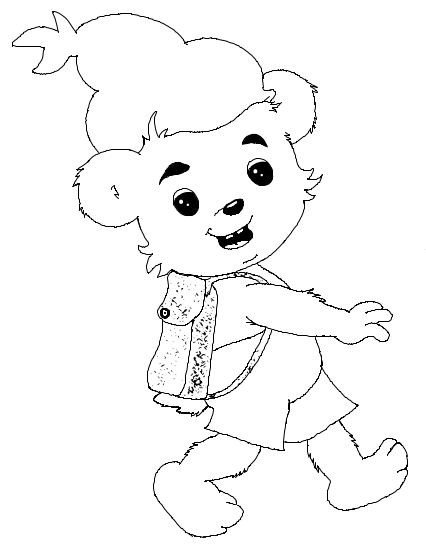
\includegraphics[width=2.7cm]{./bilder/majas-bilder/bamse-1.png}}
    %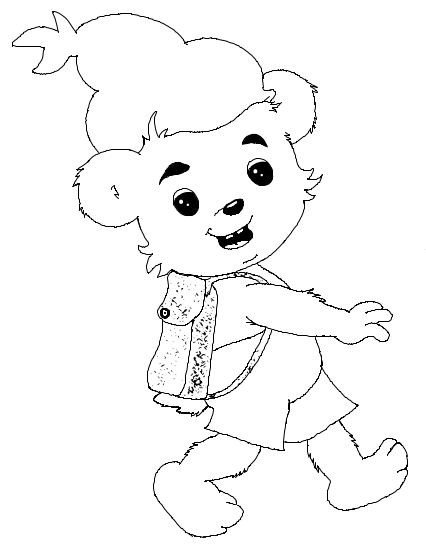
\includegraphics[width=2.4cm]{./bilder/majas-bilder/bamse-1.png}
\end{textblock*}

\begin{textblock*}{3cm}(7.5cm, 6.5cm) % {width}(x, y)
    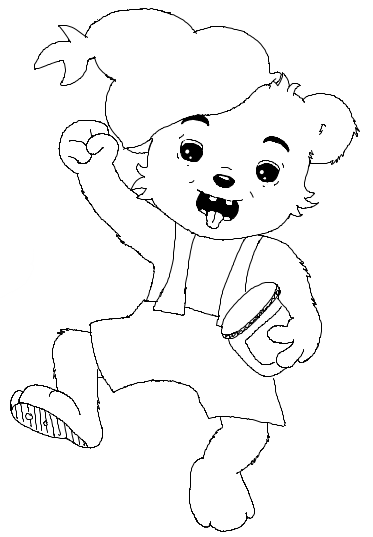
\includegraphics[width=2.4cm]{./bilder/majas-bilder/bamse-2.png}
\end{textblock*}

\begin{textblock*}{3cm}(5.7cm,10.3cm) % {width}(x, y)
    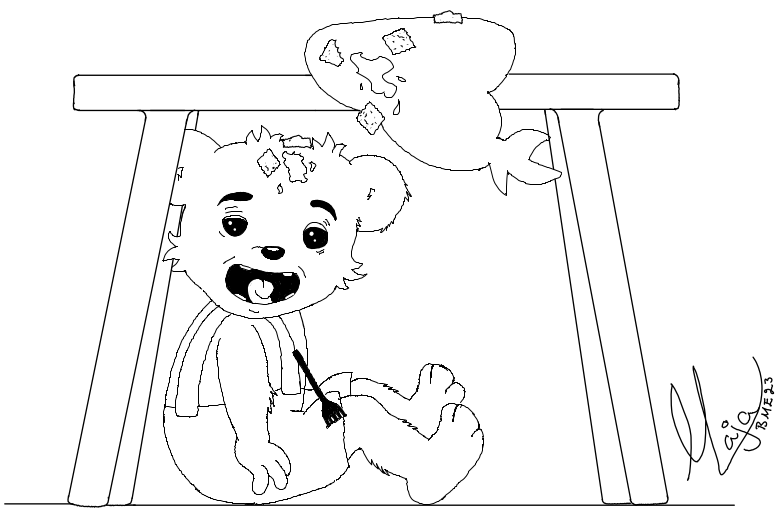
\includegraphics[width=4.2cm]{./bilder/majas-bilder/bamse-3.png}
\end{textblock*}

\subsection*{Jag skall festa} 
\index[alfa]{Jag skall festa}
\index[anfa]{Jag skall festa}
\songinfo{Mel: Bamse\\
Sångarstriden 1987}

\begin{parse lines}[\noindent]{#1\\}
    Jag ska festa, ta det lugnt med spriten,
    ha det roligt utan å va' full
    Inte krypa runt med festeliten,
    ta det varligt för min egen skull

    Först en öl i torra strupen,
    efter det så kommer supen,
    i med vinet, ner med punschen
    Sist en groggbuffé

    Jag är skitfull, däckar först av alla,
    missar festen, men vad gör väl de'?
    Blandar hejdlöst öl och gammal filmjölk,
    kastar upp på bordsdamen breve'!

    Först en öl... 

    Spyan rinner ner för ylleslipsen
    Raviolin torkar i mitt hår
    Vem har lagt mig under matsalsbordet?
    Vems är gaffeln i mitt högra lår?
\end{parse lines}

\vissteduatt{Visste du att denna sången tillsammans med Vikingen var de\\första sångerna som lades in i denna upplagan av sångboken?}

\newpage
\resetBackground

\subsection*{Ångestvisan} 
\index[alfa]{Ångestvisan}
\index[anfa]{Ångestvisan}
\songinfo{Mel: Mössens julafton}

% \colorbox{yellow}{OSÄKER PÅ DENNA}

\begin{parse lines}[\noindent]{#1\\}
    Jag vaknar upp på söndan
    och bakis som ett djur
    så kommer minnen om att gårdagskvällen spårat ur
    Jag blev visst lite busig av humle och av malt,
    på snapchatstoryn har jag publicerat allt

    Fan då, jävlar, bakfyllepanik!
    För storyn min har blivit till en eländesfabrik
    Fan då, jävlar vad ska jag ta mig till?
    För allt där finns ju sparat vare sig jag vill!

    Jag hångla med min granne
    och fast det ej va rätt,
    så sålde jag hans möbler och hans katt på internet
    Jag känner mig så rutten, jag är så full av skam
    Av alla jävla bilder på min instagram!

    Fan då, jävlar…

    Jag badade i sjön Sjøn
    och till min stora skräck,
    så fick en barnfamilj bevittna när jag dansa näck
    Jag ramlade in i bastun, och spydde upp all gin
    och likea alla exets bilder på LinkedIn

    Fan då, jävlar…
\end{parse lines}

\newpage

\subsection*{Jesus lever} 
\index[alfa]{Jesus lever}
\index[anfa]{Jesus lever}
\songinfo{Mel: Sån’t är livet}

\begin{parse lines}[\noindent]{#1\\}
    Jesus lever, han bor i Skövde
    Han kör en Volvo och han är gift
    Han har en villa med rododendron
    Han sparar pengar och jobbar skift

    Redan på lekis var han märklig
    Han ville inte leka krig
    Men när hans kompis, Knut, blev skjuten
    så lät han Jesus uppväcka sig

    Jesus lever, han bor i Skövde...

    Han gick i skolan, som alla andra
    Han var rätt duktig på gymnastik
    å vilken kille han gick på vatten
    en gång så gick han till Reykjavik

    Jesus lever, han bor i Skövde...

    I sina tonår så var han poppis
    Och han blev bjuden på varje fest
    Å vilken kille, han fick ju vatten
    att bli till rusdryck utan jäst

    Jesus lever, han bor i Skövde...
\end{parse lines}

\vissteduatt{Visste du att E-sektionen har en egen E-wiki?}
\newpage

\subsection*{Fyllevisa} 
\index[alfa]{Fyllevisa}
\index[anfa]{Jesus lever}
\songinfo{Mel: Vi går över daggstänkta berg}

\begin{parse lines}[\noindent]{#1\\}
    Vi som oss för att glupa satt, supa glatt,
    ity den, som försmår sin första tår, törsta får
    Av längtan vi tryckas
    av trängtan att lyckas
    Vi nu med bravur häller ur,
    eller hur?

    Vi ger titt som tätt strupen sitt: Supen stritt
    skall forsa, och snart får sig tarmen vår, varm en tår
    Er öven i seder
    och söven er neder
    vid denna protest-bullerfest:
    Full är bäst!
\end{parse lines}


\newpage

\subsection*{Mat och vin och öl och sprit} 
\index[alfa]{Mat och vin och öl och sprit}
\index[anfa]{Mat och vin och öl och sprit}
\songinfo{Mel: She’ll Be Coming ‘Round the Mountain\\
F-sektionen Sångarstriden 07/08}

\noindent Mat och vin och öl och sprit serveras här,\\
\noindent teknologer lider inte av misär\\
\noindent Fatta glasen och höj hatten,\\
\noindent drick nu upp den sista slatten\\
\noindent Mera vin och öl och sprit det kommer här!\\

\noindent \textit{Trula:}\\
\noindent Bordsherren min han verkar ganska snäll, \textit{(Jättesnäll!)}\\
\noindent men han beter sig lite underligt ikväll \textit{(Just ikväll!)}\\
\noindent När han glufsar i sig maten,\\
\noindent rapar högt och krossar faten\\
\noindent Tafsar han på mig då får han sig en smäll!\\

\noindent \textit{Truls:}\\
\noindent Bordsdamen min är faktiskt riktigt grann, \textit{(Jättegrann!)}\\
\noindent men hon halsar i sig ölen som en man \textit{(Vilken man?!)}\\
\noindent Vinglar hon så välter stolen,\\
\noindent Shakear loss och tappar kjolen\\
\noindent Bäst att låtsas att vi inte känt varann!\\

\noindent Mat och vin och öl och sprit serveras här...\\

\vissteduatt{Visste du att vid höstterminsmötet 2013 höll E-sektionen på att\\
 köpa en Zamboni?}

\newpage

\subsection*{Man kan dricka vatten} 
\index[alfa]{Man kan dricka vatten}
\index[anfa]{Man kan dricka vatten}
\songinfo{Mel: Vi äro musikanter}

\begin{parse lines}[\noindent]{#1\\}
    Man kan dricka vatten, mjölk och gammalt flott
    Men vi dricker hellre sådant som är gott

    Vi kan dricka brännvin, öl och billigt vin
    Vi kan dricka olja och bensin

    Och vi kan svepa islandshästar, mockavästar när vi festar
    Vi kan svepa svavelsyra på vår yra fest

    Vi kan häva kvicksilver och helium
    Vi kan häva ost och vardagsrum

    Och vi kan supa bomfadderalla, bomfadderalla,
    skål på Er alla!
    Vi kan supa andra hållet, andra hållet med
\end{parse lines}

\vissteduatt{Visste du att denna sångbok är skriven i \LaTeX?}

\newpage

\subsection*{Baklängesfyllan} 
\index[alfa]{Baklängesfyllan}
\index[anfa]{Baklängesfyllan}
\songinfo{Mel: Rövarnas visa\\
Lundakarnevalen 2018}

\begin{parse lines}[\noindent]{#1\\}
    Jag hulkar mig i spyorna
    Och sedan med en gaffel
    Ur munnen min jag plockar fram
    En extra stor falafel
    
    Sen baklänges jag vinglar bord
    Till efterfest av bästa sort
    Jag spottar ut shot, efter shot, efter shot
    ja så här finemang har jag aldrig mått!
    
    (Å shot, shot, shot, shot. Å shot, shot, shot, shot.)
    
    Till Lundagård jag rullar sen 
    Och ställer någons cykel
    På klubbens dansgolv hittar jag
    Min plånbok och min nyckel
    
    Fem öl, sju snaps, en flaska vin
    Jag häller upp ur halsen min
    Ikväll ska jag plugga det lovar jag dig,
    men en endaste öl kan man unna sig!
    
\end{parse lines}

\newpage


\begin{textblock*}{3cm}(8.5cm,-0.7cm) % {width}(x, y)
    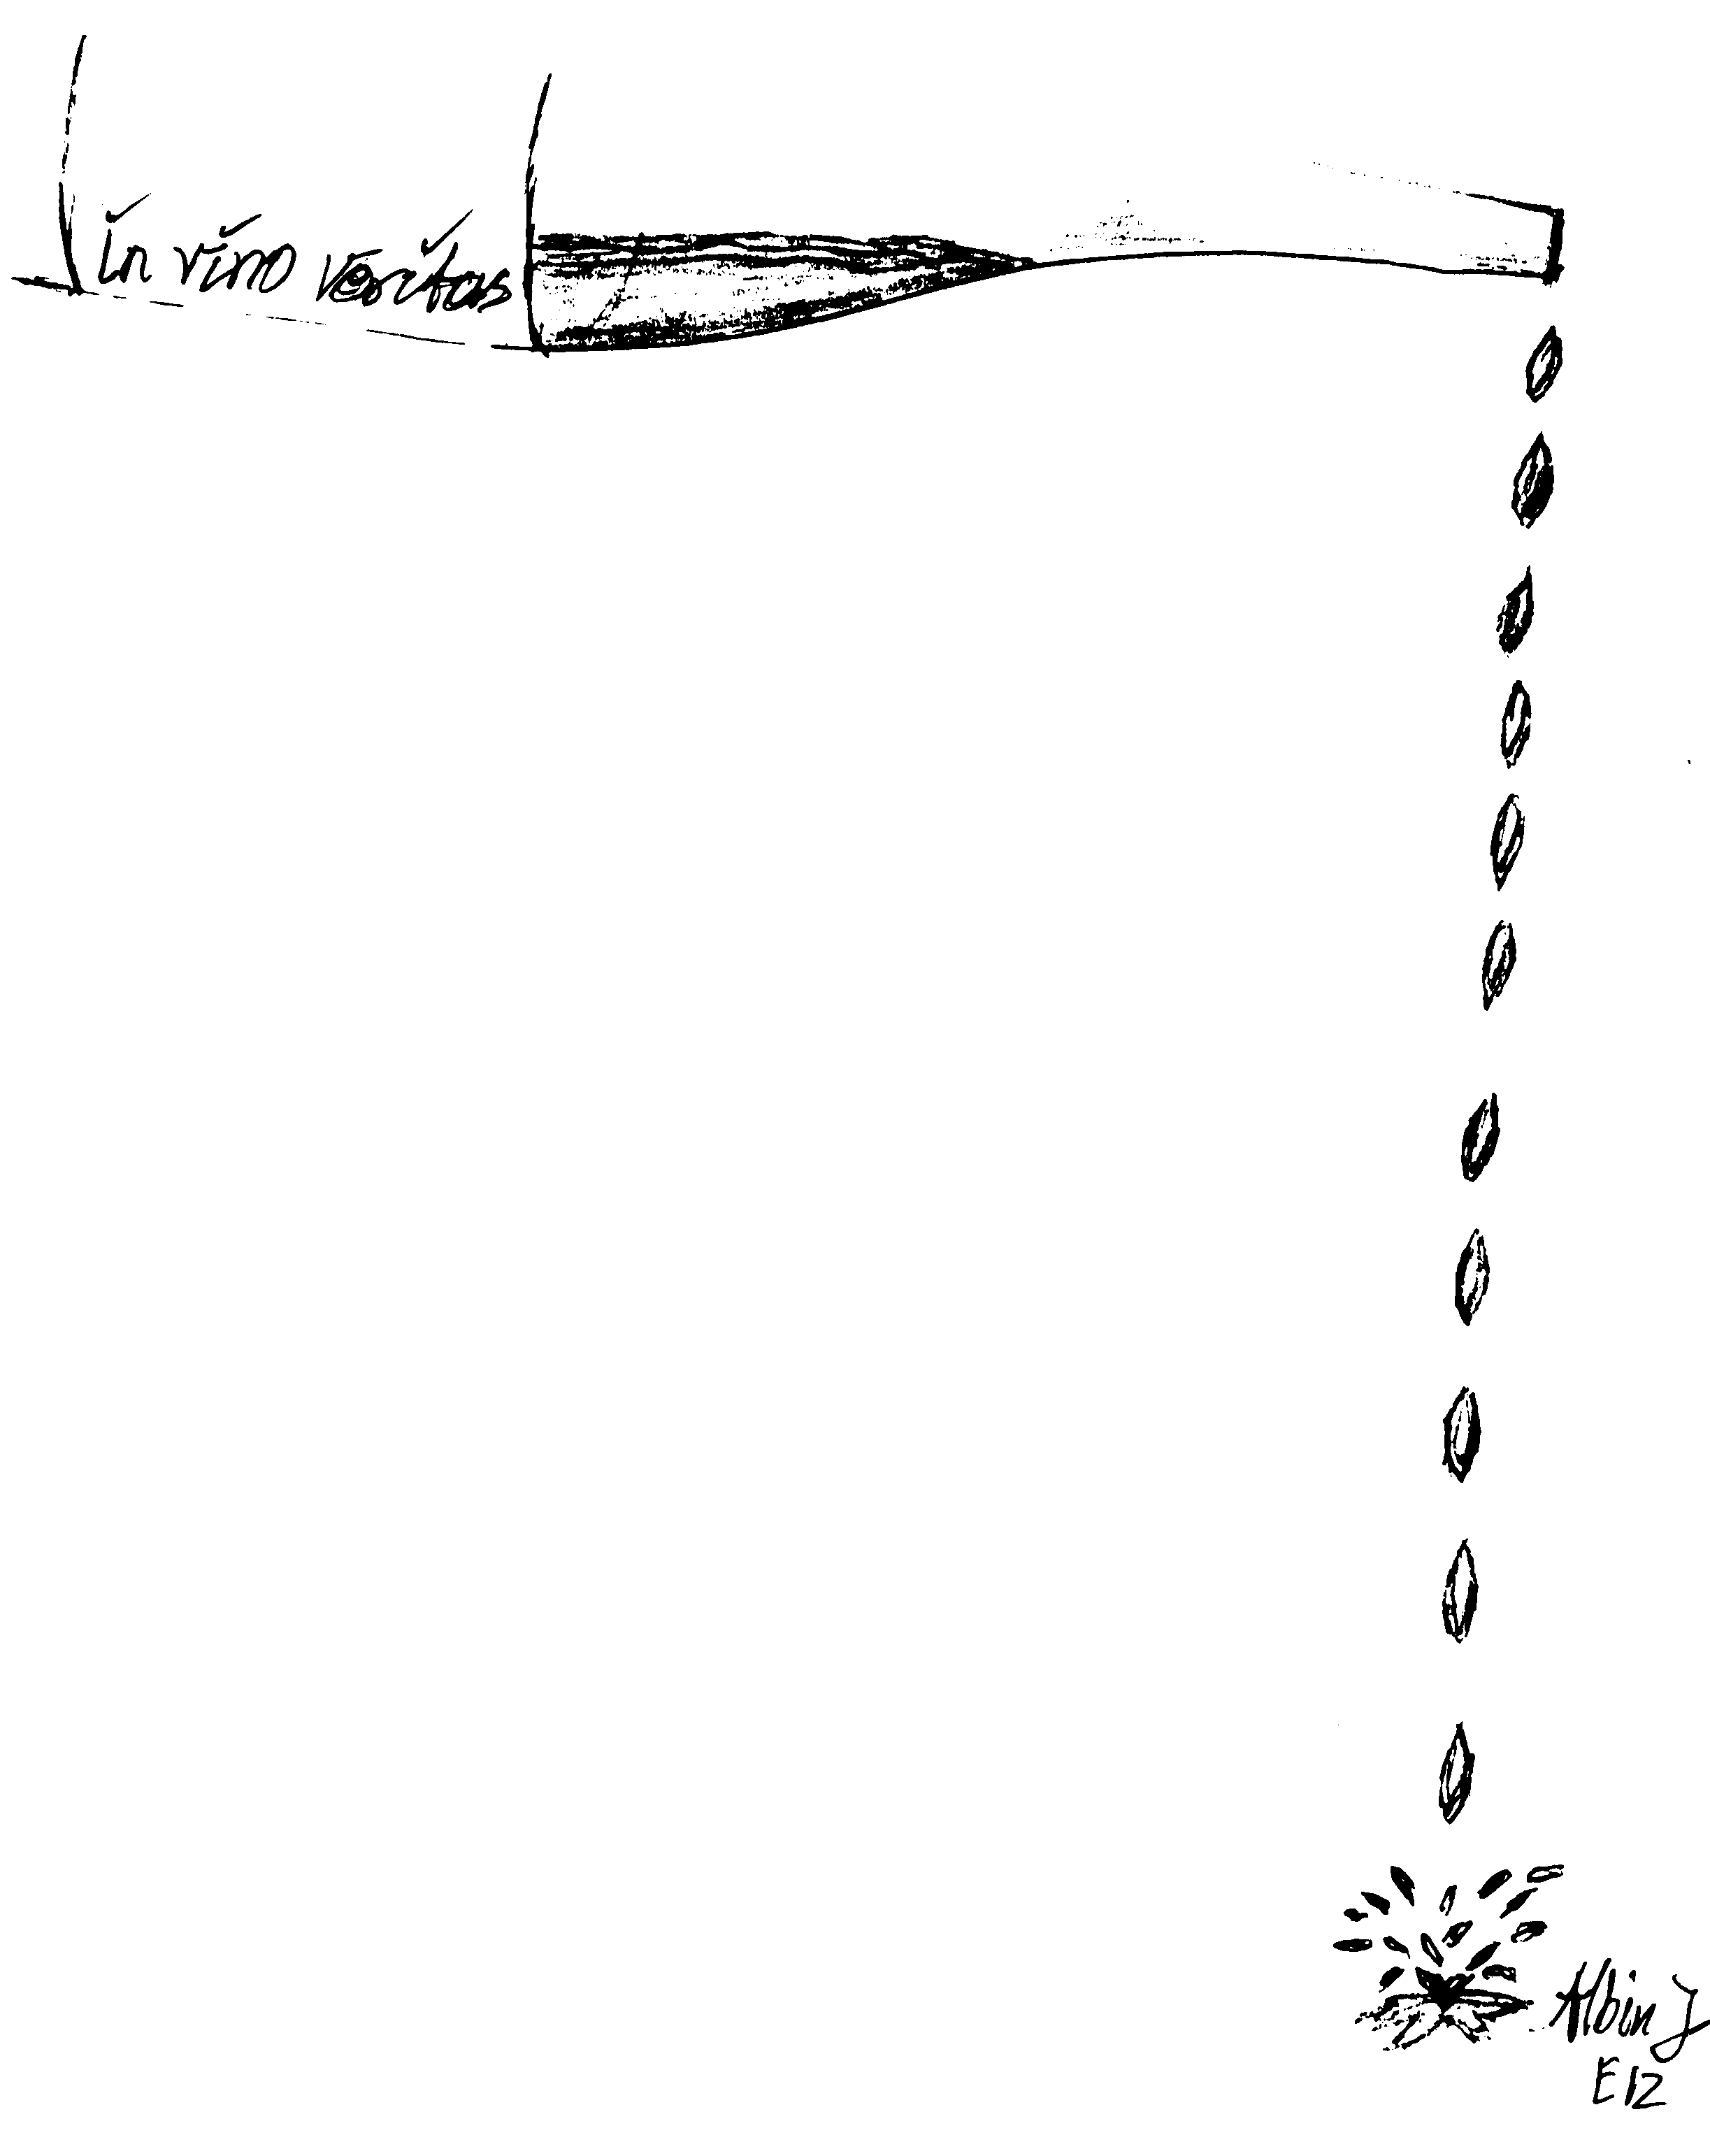
\includegraphics[width=12cm]{./bilder/in_vino_veritas.png}
\end{textblock*}

\subsection*{Kalmarevisan} 
\index[alfa]{Kalmarevisan}
\index[anfa]{Uti Kalmare stad}
\songinfo{Sången leds av sångförman}

\noindent \textit{Uti Kalmare stad,} \\
\noindent ja där finns det ingen kvast \\
\noindent förrän lördagen \\

\noindent \textit{Hej dick,} hej dack\\
\noindent \textit{Jag slog i,} och vi drack\\
\noindent \textit{Hej dickom dickom dack,}\\
\noindent Hej dickom dickom dack\\
\noindent För uti Kalmare stad\\
\noindent ja där finns det ingen kvast\\
\noindent förrän lördagen\\

\noindent ||: \textit{När som bonden kommer hem}\\
\noindent kommer bondegumman ut :||\\
\noindent är så stor i sin trut\\
\noindent \textit{Hej dick…}\\

\noindent ||: \textit{Var är pengarna du fått?}\\
\noindent - Jo, dem har jag supit opp :||\\
\noindent uppå Kalmare slott\\
\noindent \textit{Hej dick…}\\

\vissteduatt{Visste du att LTH-fontänen invigdes 1970 men plockades ner 1996\\efter otaliga försök att reparera den? Kvar står stålskelettet.}

\newpage
\noBackground

\begin{textblock*}{3cm}(-2.0cm,-0.7cm) % {width}(x, y)
    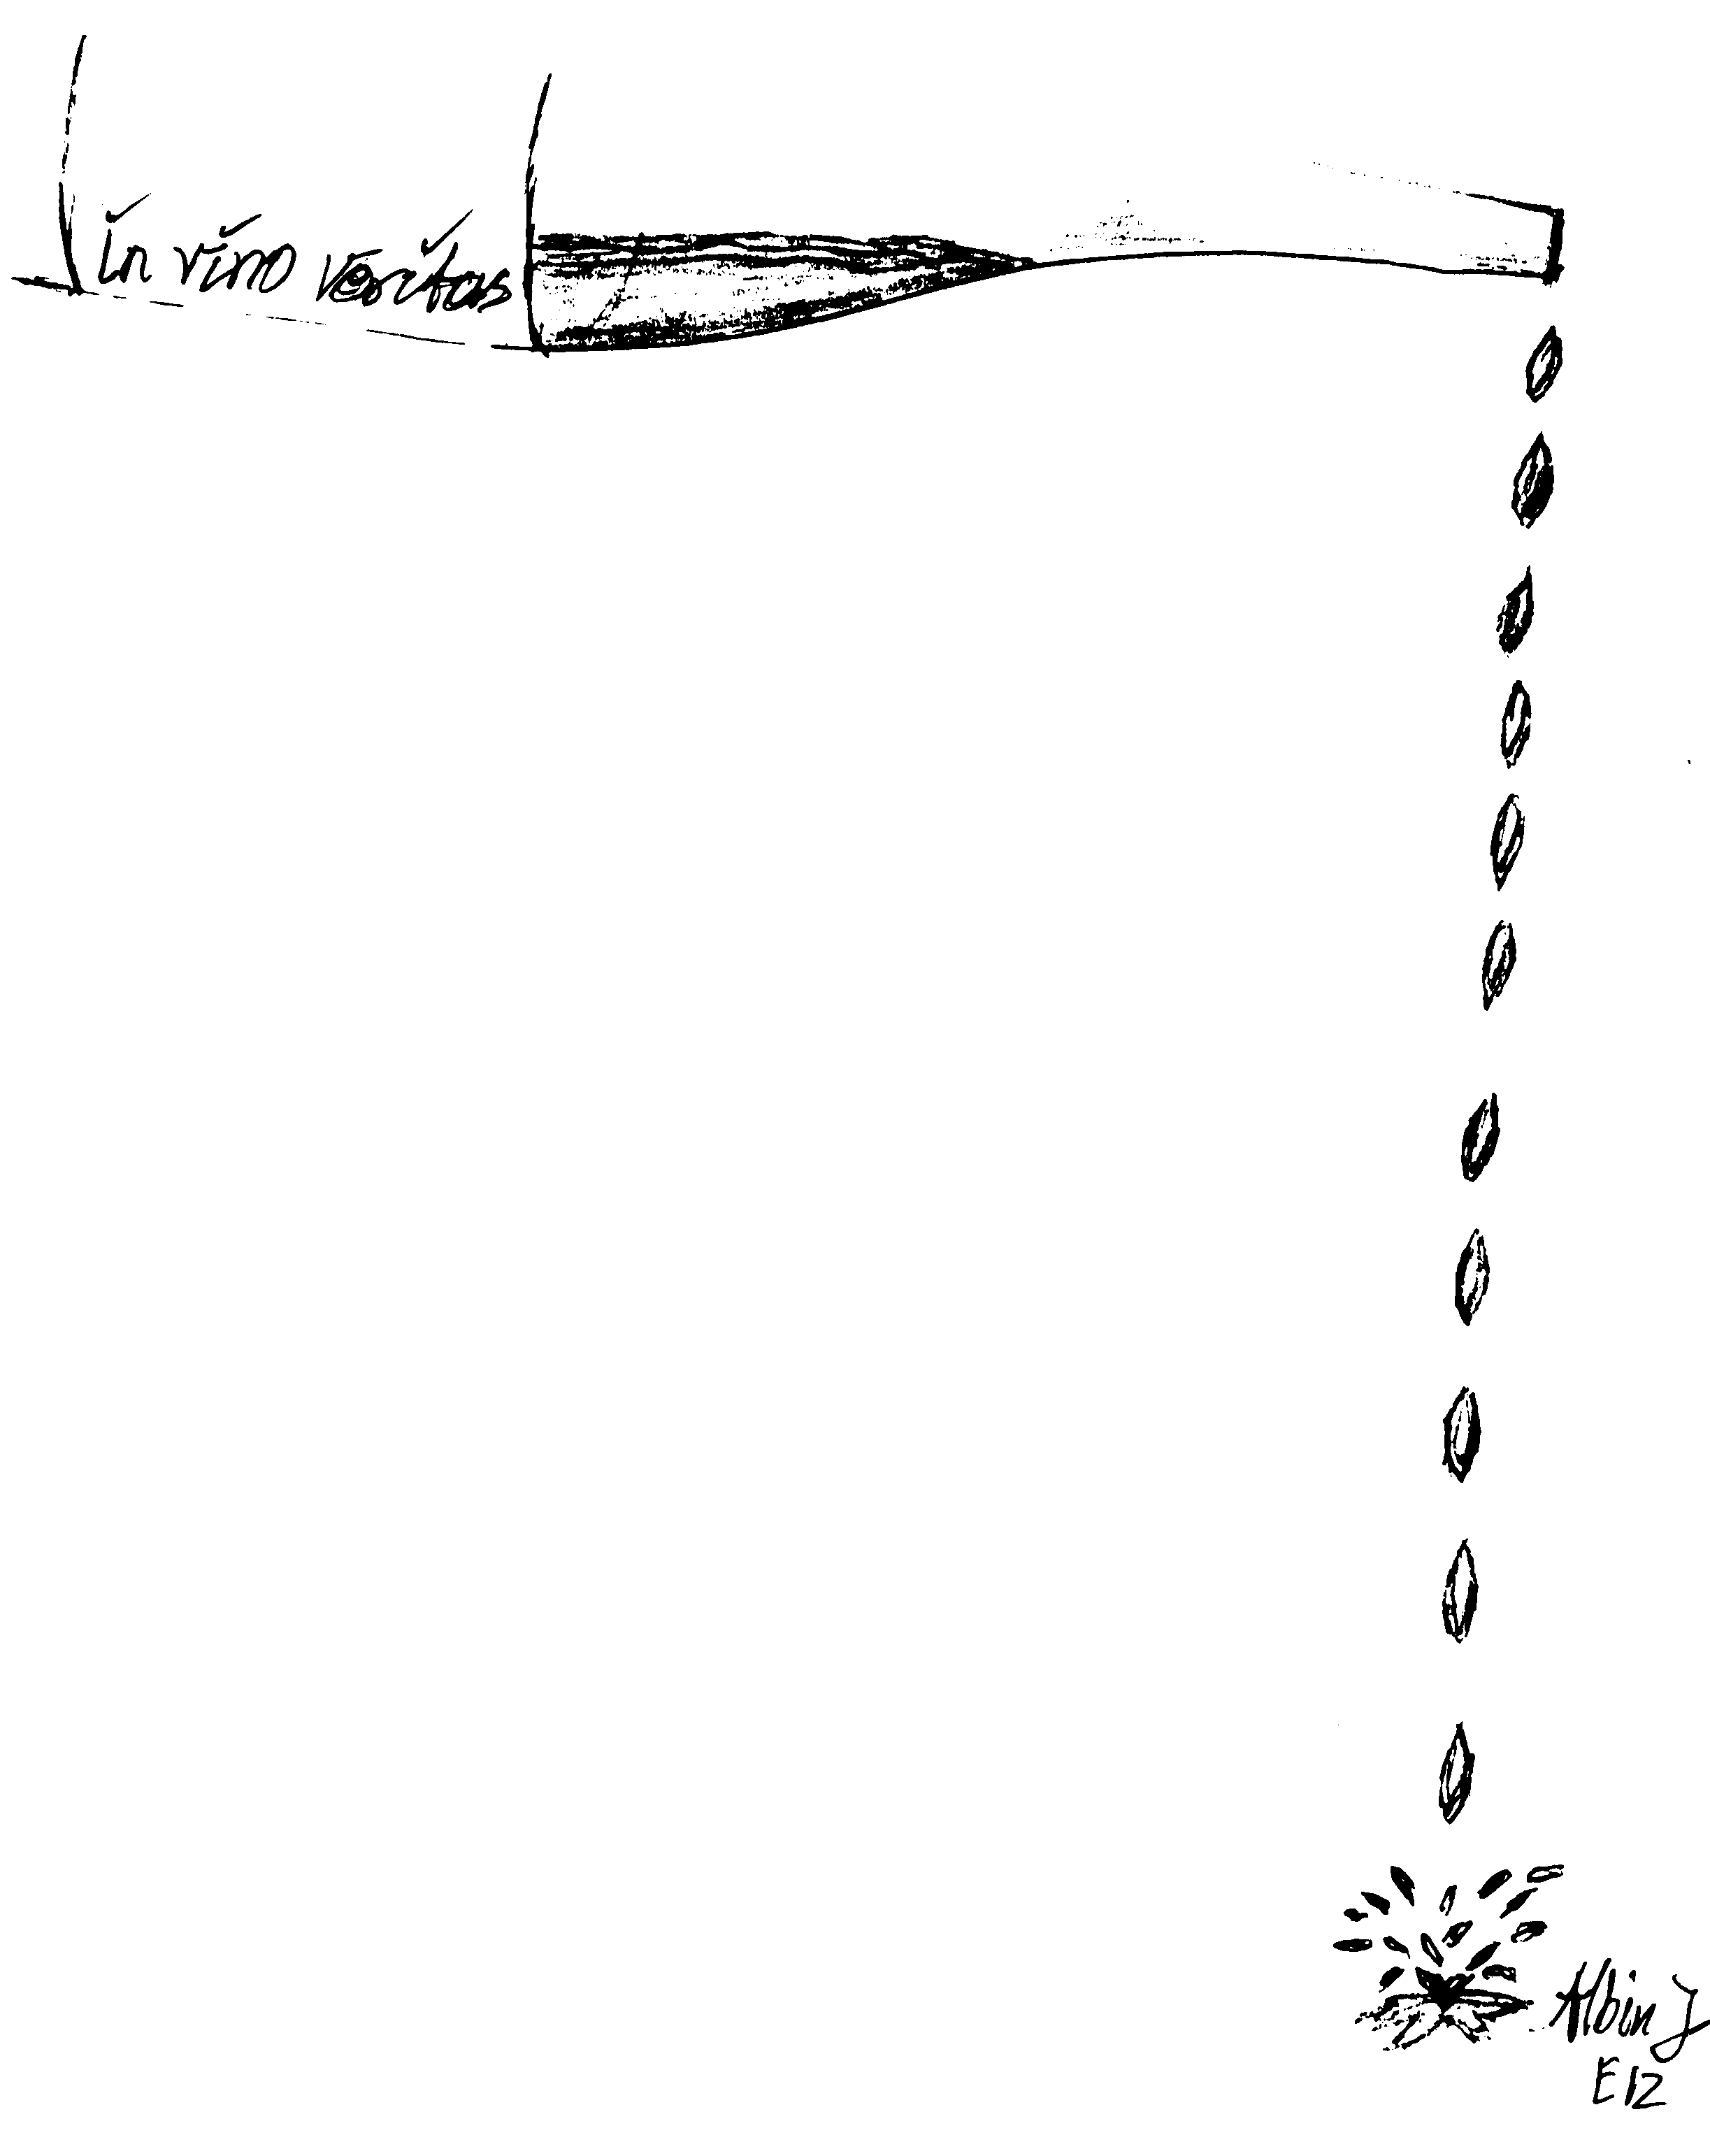
\includegraphics[width=12cm]{./bilder/in_vino_veritas.png}
\end{textblock*}

*\vspace{1cm}

\noindent ||: \textit{Jag skall klaga dig an}\\
\noindent för vår kronbefallningsman :||\\
\noindent och så får du skam\\
\noindent \textit{Hej dick…}\\

\noindent ||: \textit{Kronbefallningsmannen vår}\\
\noindent satt på krogen i går :||\\
\noindent och var full som ett får\\
\noindent \textit{Hej dick…}\\

\noindent ||: \textit{Var har du din labbrapport?}\\
\noindent Jo den har jag supit bort! :||\\
\noindent Den var allt för kort\\
\noindent \textit{Hej dick…}\\

\vissteduatt{Visste du att "In Vino Veritas"?}

\newpage

\subsection*{Spritbolaget} 
\index[alfa]{Spritbolaget}
\index[anfa]{Till spritbolaget ränner jag}
\songinfo{Mel: Snickerboa\\
Text: Göran Bolinder E87\\
E-sektionen Sångarstriden 1989}

\begin{parse lines}[\noindent]{#1\\}

    Till spritbolaget ränner jag
    och bankar på dess port
    Jag vill ha nå't som bränner bra
    och gör mig sketfull fort
    Expediten sade: Godda',
    hur gammal kan min herre va'?
    Har du nå't leg, ditt fula drägg?
    Kom hit igen när du fått skägg!
    
    Nej, detta var ju inte bra,
    jag ska bli full ikväll
    Då plötsligt en idé fick jag:
    De har ju sprit på Shell
    Många flaskor stod där på rad,
    så nu kan jag bli full och glad
    Den röda drycken åkte ner...
    Nu kan jag inte se nå't mer
\end{parse lines}

\vissteduatt{Visste du att E-sektionen bara kom på andra plats med Spritbolaget?}

\newpage
\resetBackground


\subsection*{Härjarevisan} 
\index[alfa]{Härjarevisan}
\index[anfa]{Nu ska vi ut och härja}
\songinfo{Mel: Gärdebylåten\\ Ur Lundaspexet Djingis Khan 1954\\ Text: Hans Alfredsson}

\begin{parse lines}[\noindent]{#1\\}

    Hurra! Nu ska man äntligen få röra på benen
    Hela stammen jublar och det spritter i grenen
    Tänk att än en gång få spränga fram på Brunte i galopp!
    Din doft, o käre Brunte är trots brist i hygienen,
    för en vild mongol minst lika ljuv som syrenen
    Tänk att på din rygg få rida runt i sta'n och spela topp!

    Ja, nu ska vi ut och härja,
    supa och slåss och svärja,
    bränna röda stugor, slå små barn och säga fula ord
    Med blod ska vi stäppen färga
    Nu änteligen lär jag
    kunna dra nån riktig nytta av min
    Hermodskurs i mord

    Ja, mordbränder är klämmiga, ta fram fotogenen
    Eftersläckningen tillhör just de fenomenen
    inom brandmansyrket som jag tycker det är nån nytta med
    Jag målar för mitt inre upp den härliga scenen,
    blodrött mitt i brandgult, ej prins Eugen en
    lika mustig vy kan måla, ens om han målade med sked

    Ja, nu ska vi ut och härja…

\end{parse lines}

\vissteduattlong{Visste du att det finns en tredje vers som felaktigt sjunges av \\
andra högskolor innan första versen? Originalet skrevs trots allt \\
i Lund...}

\newpage

\subsection*{Smögen} 
\index[alfa]{Smögen}
\index[anfa]{Kärlek och solsken och sång}
\songinfo{Mel: När jag var en ung caballero}

\begin{parse lines}[\noindent]{#1\\}
    När jag vart' och spytt på kalaset 
    Så kallar dom mig fylle-..........Karlsson 
    En Karlsson för kärlek och solsken och sång, 
    för kärlek och solsken och sång, PLING PLONG 
    
    Så ramla jag på någon Trula 
    Och vi börja genast att .......... prata 
    Prata för kärlek… 
    
    Hon sade att hon hette Ulla 
    och fråga om vi skulle .......... dansa 
    
    Hon ville att jag ville titta 
    på hennes förtjusande .......... våning 
    En våning för kärlek… 
    
    Hon ville att jag ville titta 
    på hennes förtjusande .......... våning 
    En våning för kärlek… 
    
    Hon sa: “Här é vackert om hösten” 
    och smekte de fylliga .......... bolstren 
    Det var bolster för kärlek… 
    
    Som förrätt, hon sa “får väl duga 
    att vi varann häftigt kan .......... krama” 
    Det var kramar för kärlek… 
\end{parse lines}
\enlargethispage{1cm}
\newpage
\noBackground

\begin{textblock*}{3cm}(1cm,10.3cm) % {width}(x, y)
    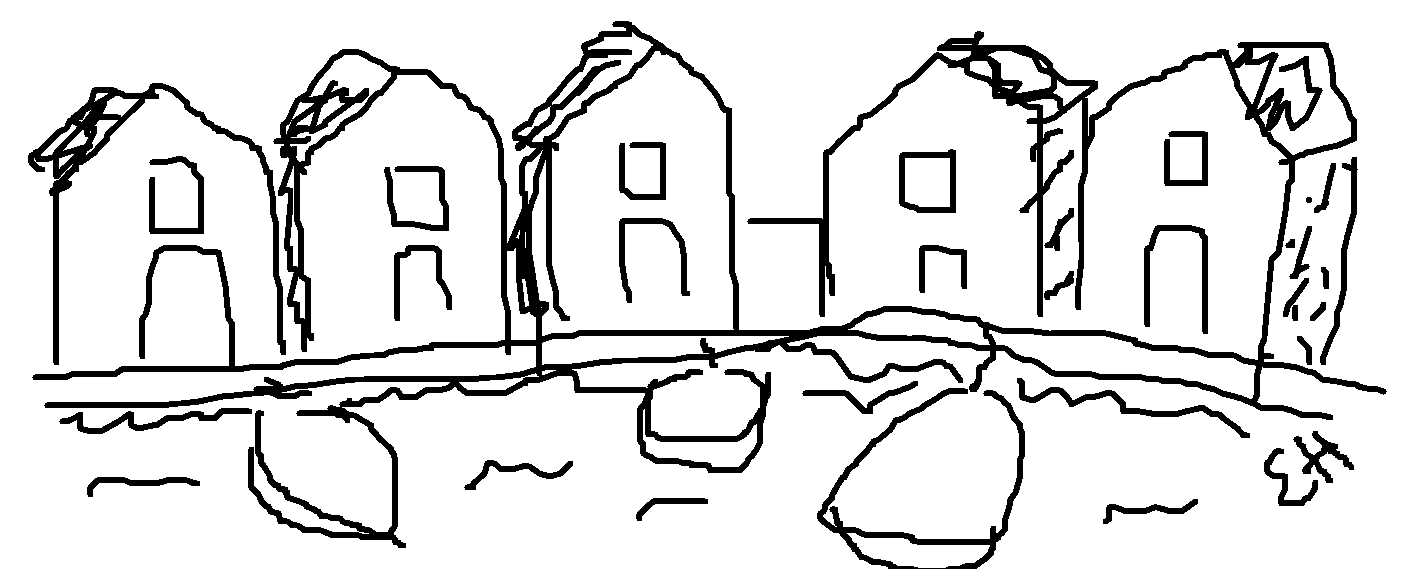
\includegraphics[width=8.5cm]{./bilder/smogen.png}
\end{textblock*}

\begin{parse lines}[\noindent]{#1\\}
    Hon bjöd mig på kaffe och tårta 
    och vi blev så helvetes .......... mätta 
    Vi va mätta på kärlek… 
    
    Så spillde jag kaffe på duken 
    jag torkade upp det med .......... trasan 
    En trasa för kärlek… 
    
    Då kom hennes storebror Östen 
    Han bad henne visa mig .......... tavlan 
    En tavla för kärlek… 
    
    Så tog hon av sig till mitten, 
    och jag börja fumla med .......... TVn 
    En TV för kärlek… 
    
    Sen börja vi ekorrar härma 
    när jag fyllde henne med .......... nötter 
    Det var nötter för kärlek… 
    
    Sen börja jag hemåt att lunka 
    Jag stanna i porten och .......... gäspa 
    Jag gäspa för kärlek…

\end{parse lines}
\vissteduatt{\\Visste du att den här bilden ritades på 2 minuter i MS Paint?}
\newpage
\resetBackground

\subsection*{Antisnapsvisa} 
\index[alfa]{Antisnapsvisa}
\index[anfa]{Huvudet vi lyfter med ett stön ur vår säng}
\songinfo{Mel: Sjösala vals}

\begin{parse lines}[\noindent]{#1\\}
    Huvudet vi lyfter med ett stön ur vår säng,
    tvättmaskin i buken, kanoner i huvudet.
    Tungan som en plyschsoffa och yrseln i sväng,
    i ångesten vi svettas 
    kom sjung din refräng:

    Varför finns det aldrig nå'n nykter karneval?
    O, låt oss somna om så vi slipper våra kval
    men se så många supar vi redan kastat upp i sängen:
    Renat och Skåne, Svart Vinbär och fager Bäsk
\end{parse lines}

\subsection*{Katastrofalt uppvaknande} 
\index[alfa]{Katastrofalt uppvaknande}
\index[anfa]{Jag vaknade i stolen}
\songinfo{Mel: Stad i ljus\\
Lundakarnevalen 2022}

\begin{parse lines}[\noindent]{#1\\}
    Jag vaknade i stolen, har slumrat till här i mitt rum
    Och allting känns eländigt, mitt bord är fyllt med 
    flaskor - en har runnit ut
    Jag tror jag minns spektaklet och alla dom som 
    förde liv
    Konturen av ett party, jag hade efterfest som växte -
    blev massiv

    Jag är full!
    i ett kaosartat rum
    Ge mig frid
    så jag får somna om
\end{parse lines}

\vissteduatt{Visste du att vid höstterminsmötet 2021 höll E-sektionen på att köpa\\in en åkbar sopmaskin och bygga om halva Edekvata till garage?}
\newpage
\noBackground

\begin{textblock*}{3cm}(2.8cm,7.2cm) % {width}(x, y)
    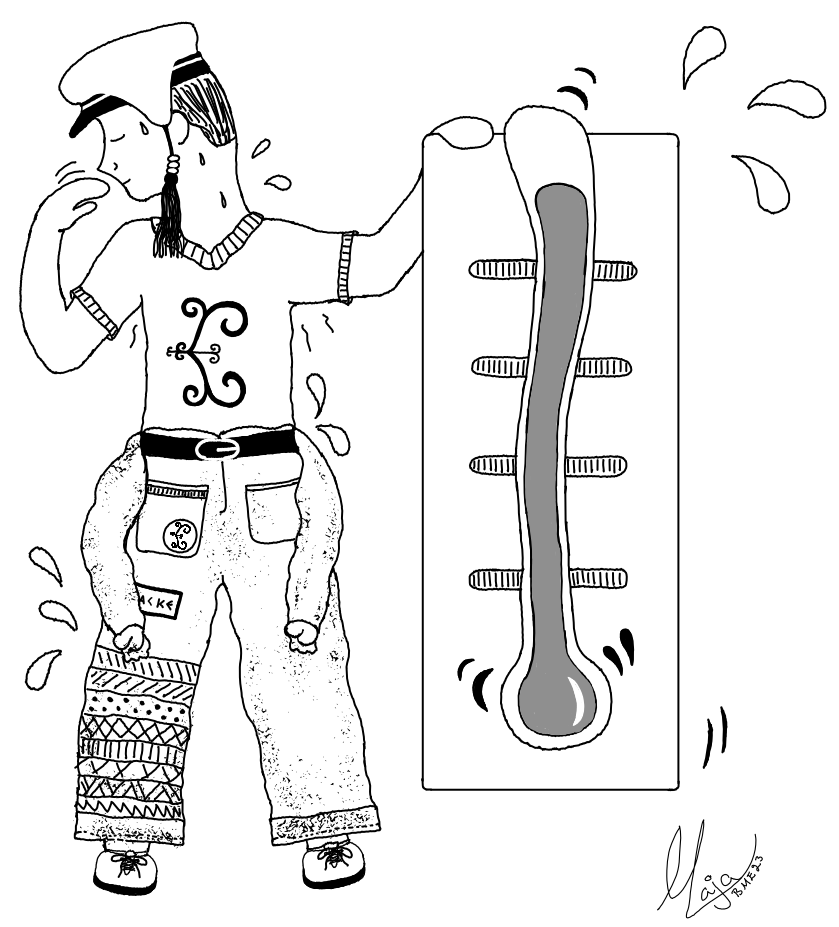
\includegraphics[width=6cm]{./bilder/majas-bilder/temperaturen.png}
\end{textblock*}

\subsection*{Temperaturen} 
\index[alfa]{Temperaturen}
\index[anfa]{Temperaturen}
\songinfo{Text: Mora Träsk}

\begin{parse lines}[\noindent]{#1\\}
    När temperaturen är hög uti kroppen
    Närmare 40 än trettiosju komma fem
    Så ska det vara när ångan är uppe
    och så är fallet uti detta nu

    Vi rullar, vi rullar…

    August och Lotta…

    Framåt och bakåt…

    ...
\end{parse lines}

\newpage